\begin{frame}{\insertsection}{Original proposal by Kim, Kwon and Park}
	\begin{columns}[T]
	\column{0.5\textwidth}
	\begin{itemize}
	\item three-level pyramid decomposition
	\item watermark embedding in all sub-bands except $LH_1$, $HL_1$, $HH_1$
	\newline \textcolor{TUDblue}{$\Rightarrow$} low energy in those bands
	\item multi-resolution for robustness
	\item embedding strength proportional to band energy
	\end{itemize}
	\column{0.5\textwidth}
	\centering
	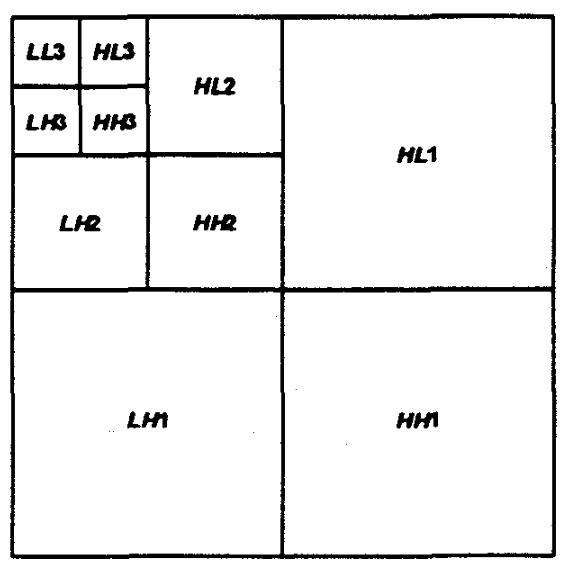
\includegraphics[width=.8\textwidth]{Bilder/threelayerMotivation} 
	
	DWT decomposition (\cite{779947})
	\end{columns} 	
\end{frame}

\begin{frame}{\insertsection}{Implemented method}
	\begin{columns}[T]
	\column{0.5\textwidth}
	\begin{itemize}
	\item Daubechies filter used for DWT
	\item three-level pyramid decomposition
	\item watermark embedding in high resolution sub-bands $LH_3$, $HL_3$, $HH_3$ 
	\item embedding strength $\alpha_i$
	\newline \textcolor{TUDblue}{$\Rightarrow$} robustness vs. imperceptibility %chosen that $\text{PSNR} = \SI{45}{\deci\bel}$
	\item each sub-band $B$ has $N_B = 4096$ coefficients 
	\newline \textcolor{TUDblue}{$\Rightarrow$} watermark size $N = 12288$
	\item multiplicative embedding	
	\newline \textcolor{TUDblue}{$\Rightarrow$} $y_i = x_i(1+\alpha_iw_i)$
	\end{itemize}
	\column{0.5\textwidth}
	\centering
	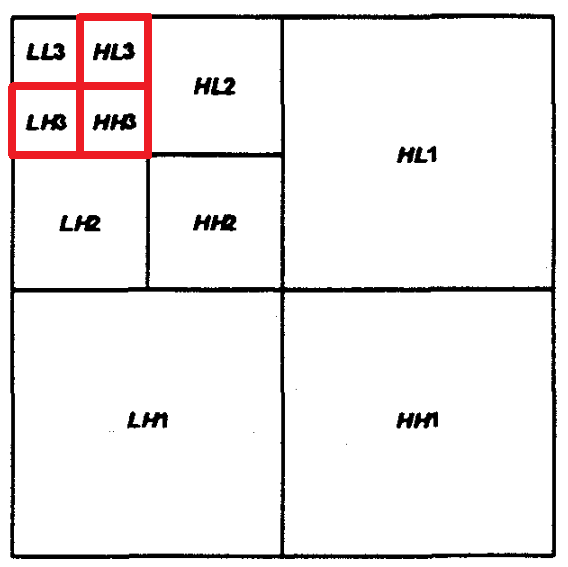
\includegraphics[width=.8\textwidth]{Bilder/threelayerMotivationPainted} 
	
	DWT decomposition with used sub-bands 
	\end{columns} 	
\end{frame}

\begin{frame}{\insertsection}{Implemented method}
	\begin{columns}[T]
	\column{0.5\textwidth}
	\begin{itemize}
	\item each sub-band $B$ has $N_B = 4096$ coefficients 
	\newline \textcolor{TUDblue}{$\Rightarrow$} watermark size $N = 12288$
	\item Watermarks are i.i.d. $\mathcal{U}(-1, 1)$
	\item Original sub-bands i.i.d., assumed to be Laplacian distributed
	\item No correlation between sub-bands assumed
	\end{itemize}
	\column{0.5\textwidth}
	\centering
	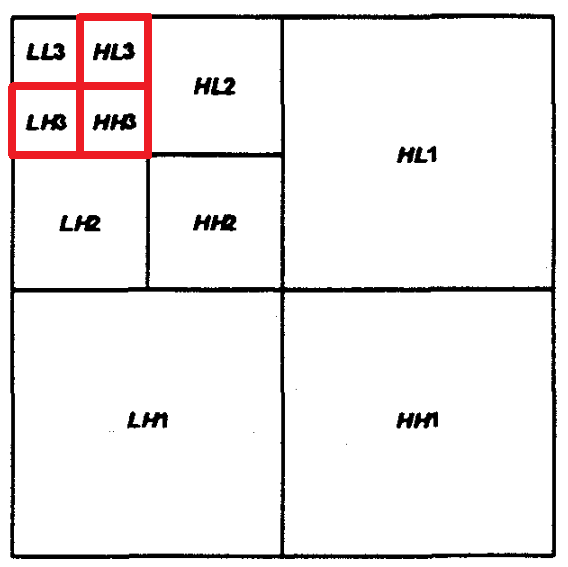
\includegraphics[width=.8\textwidth]{Bilder/threelayerMotivationPainted} 
	
	DWT decomposition with used sub-bands 
	\end{columns} 	
\end{frame}